\subsection{Test Configuration}

DEF is designed to be transparently compatible with C in that C header files can be included in DEF, and the utility \texttt{defghi} (DEF Generate Headers and Interfaces), can take DEF source files and emit C header files for inclusion in C.  This makes it easy to correct for any variation created by the benchmark driver or the allocator.



\begin{figure}
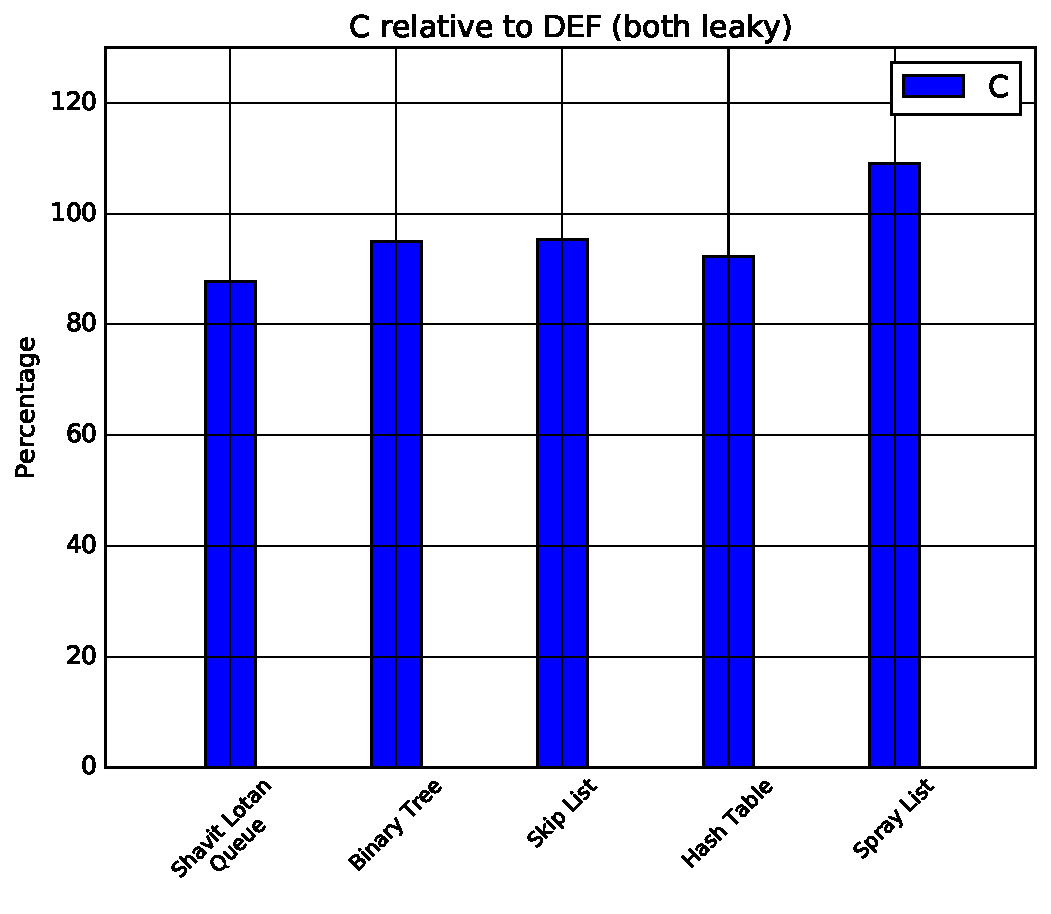
\includegraphics[scale=0.4]{gfx/relativeperf.pdf}
\caption{Relative performance of C to DEF}
\end{figure}
\begin{figure}
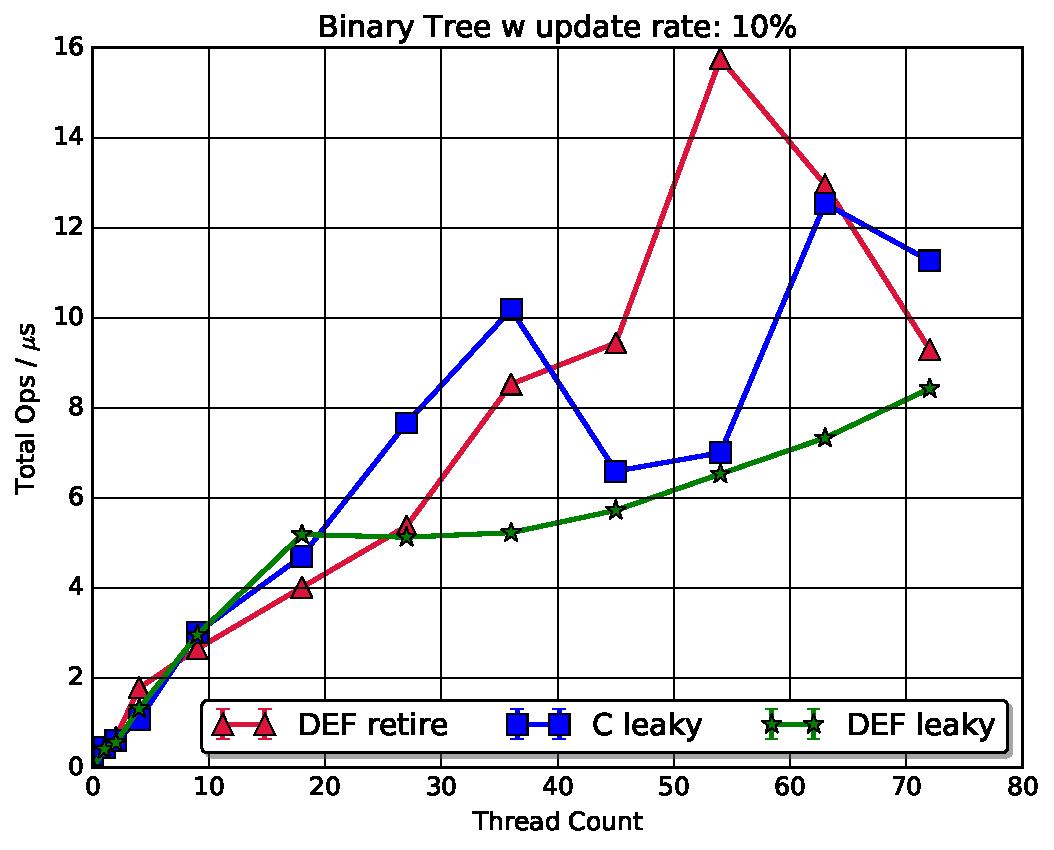
\includegraphics[scale=.4]{gfx/BinaryTreeLight.pdf}
\caption{Lock-Free Binary Tree}
\end{figure}

\begin{figure}
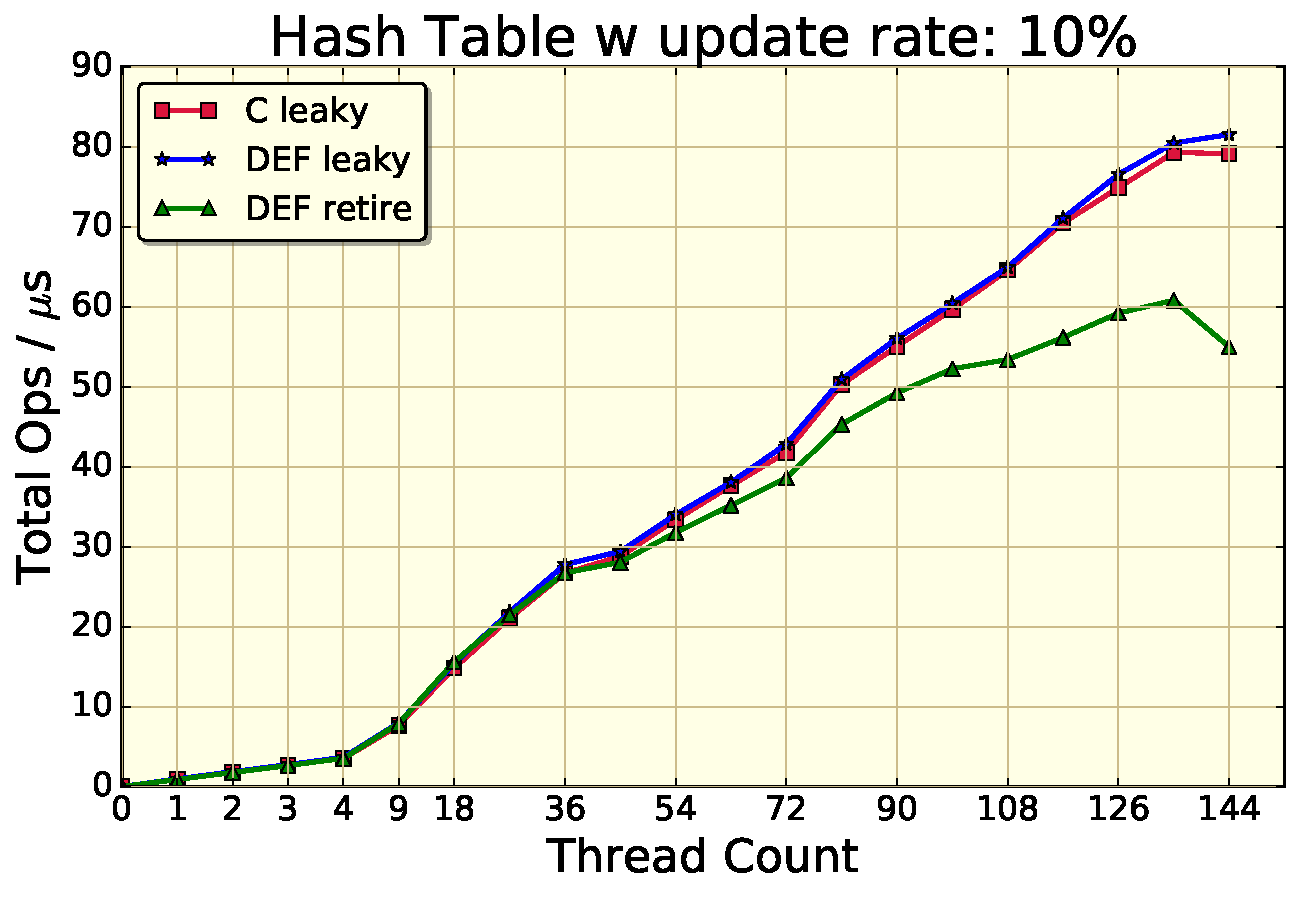
\includegraphics[scale=.4]{gfx/HashTableLight.pdf}
\caption{Lock-Free Hash Table}
\end{figure}

\begin{figure}
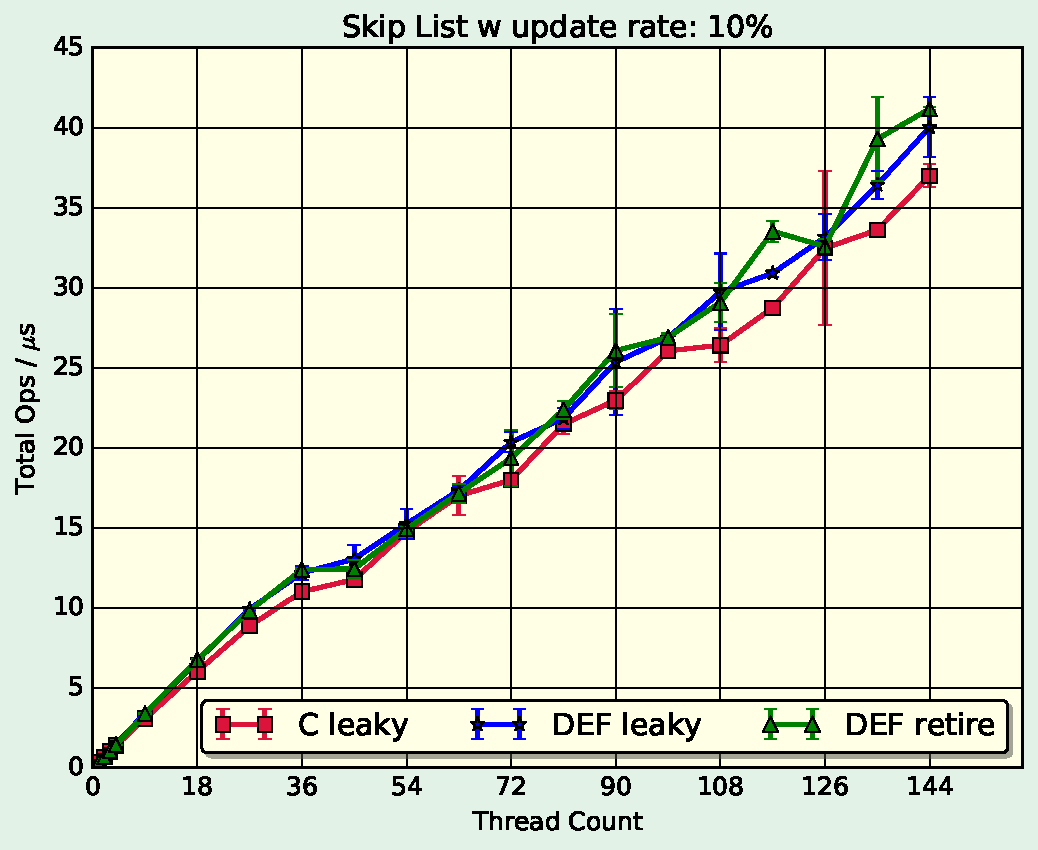
\includegraphics[scale=.4]{gfx/SkipListLight.pdf}
\caption{Lock-Free Skip List}
\end{figure}

\begin{figure}
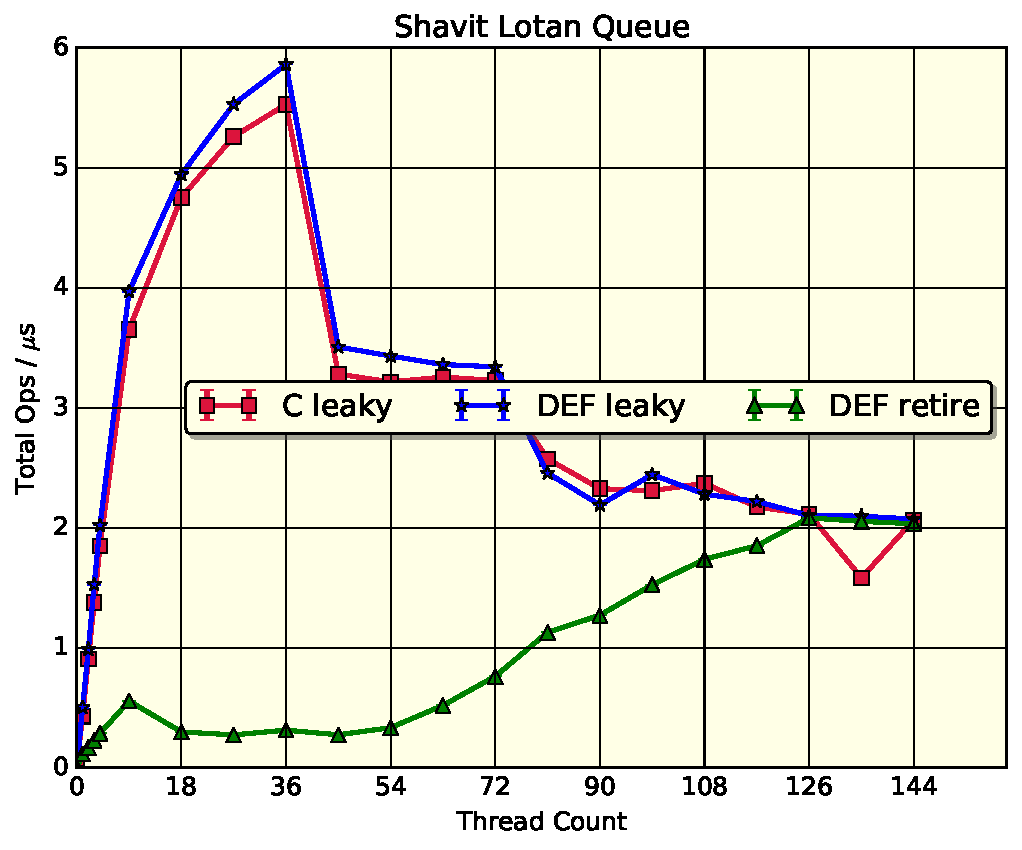
\includegraphics[scale=.4]{gfx/ShavitLotanQueue.pdf}
\caption{Lock-Free Priority Queue}
\end{figure}

\begin{figure}
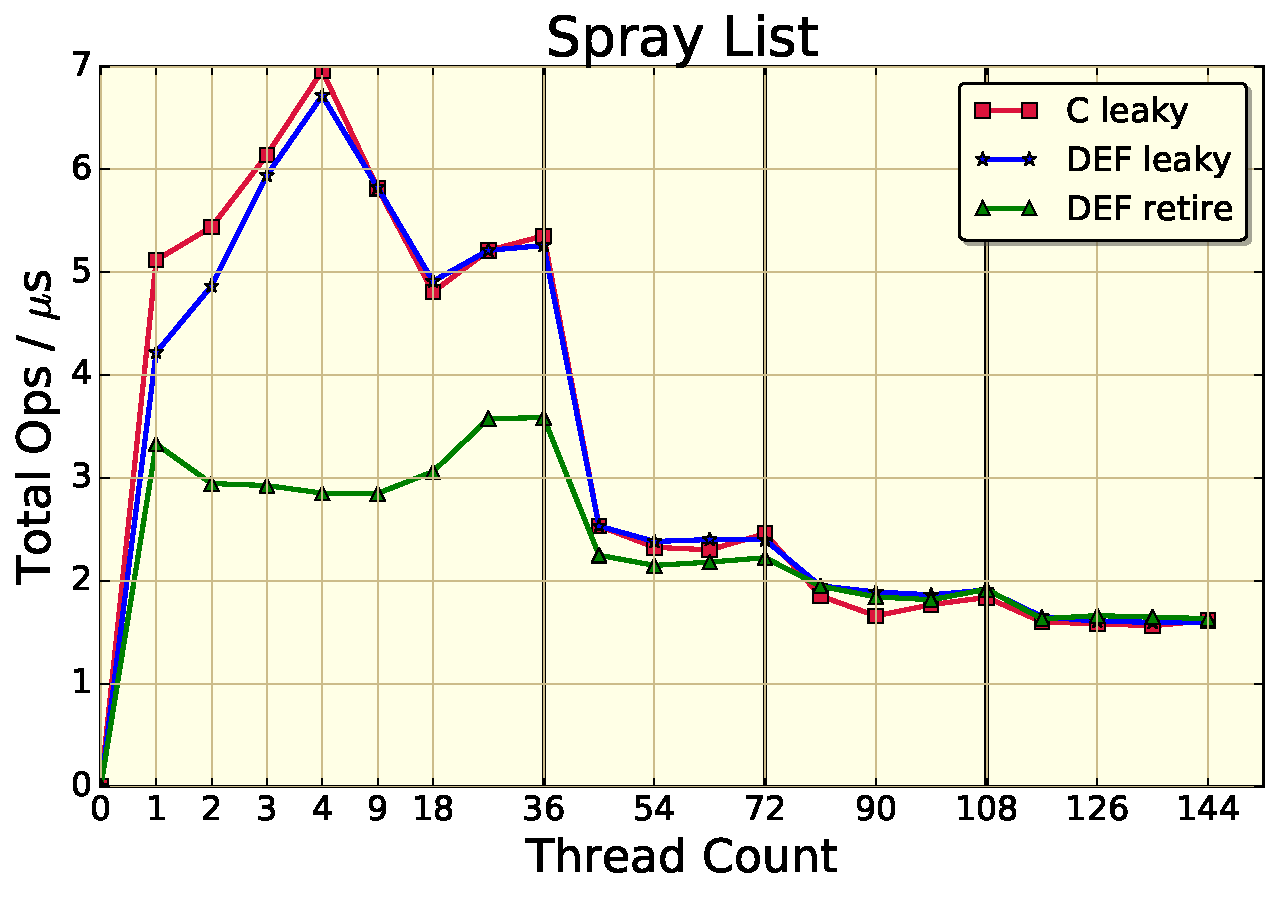
\includegraphics[scale=.4]{gfx/SprayList.pdf}
\caption{Spray List Priority Queue}
\end{figure}

\subsection{Experimental Results}
